\documentclass[11pt]{amsart}
%%% WARNING: Do NOT change the page size, fonts, or margins!  Penalties will apply.


\usepackage{graphicx}
\usepackage{amssymb,amsmath,amsthm}
\usepackage{placeins} %enables \FloatBarrier, that prevents floats from going below it.
\usepackage{caption}
\usepackage{subcaption}
\usepackage{tikz}
\usepackage{physics}
\usetikzlibrary{arrows}
\usetikzlibrary{tikzmark}

%%% WARNING: Do NOT change the page size, fonts, or margins!  Penalties will apply.
%%% WARNING: Do NOT change the page size, fonts, or margins!  Penalties will apply.

% Some macros for ease of use
\newcommand{\R}{{\mathbb R}}
\newcommand{\A}{{\mathrm{A}}}


\begin{document}

\title{Modeling BYU Math Migration}
\author{Cannon Tuttle, Curtis Evans, Taylor Jones}

%% comment out next command to put today's date after names of group members, or put a desired day in the parethesis
\date{}

\maketitle

\begin{abstract}
    This project delves into modeling the migration patterns of BYU Math students using a three-patch 
    system to represent their presence in the Math Lab, classrooms, or elsewhere on campus. The focus is on creating 
    a model specifically targeting the Math Lab to look at the dynamics of student migration towards it. 
    Our goal is to provide Math Lab administrators with insights to optimize tutor scheduling during peak influx periods.
    
    While the model captures a few trends, we acknowlege its limitations. The model found the largest influx of students into the Math 
    Lab occurs during the break period between classes suggesting a strategic adjustment in the scheduling of Math Lab 
    employees' shifts. We propose shifts to begin at the 30-minute mark rather than the start of the hour to 
    optimize the Math Lab's ability to manage student influxes efficiently ensuring tutors are ready to assist when 
    needed.
\end{abstract}

%% First Section
\section{Background/Motivation}



%% Second Section 
\section{Kalman Filter Alteration}
We ran into a problem of using our observation in the Kalman filter. The problem was coming around when the angles got around $0$
and $2\pi$

\subsection{Building the Model} 


\subsection{Defining the Alpha matrix}


\begin{equation*}
    \text{Let } S_{t_0,t_1,p}(t, a, b) = \begin{cases}a & \text{if } t_0 \le t\mkern-5mu\pmod{p} \le t_1\\ b& \text{otherwise}\end{cases}
\end{equation*}

By then defining the shorthands $S = S_{50, 55, 60}$ and $S_\star = S_{0, 50, 60}$
(favoring transitions between class or during class respectively)
we could finally write the following discontinuous $A$ function:




\subsection{Boundary Value Problem}
We wanted to also simulate our system ensuring that students all went elsewhere at the end of class.
For this, we used a BVP solver, but we needed to add 3 parameters to add enough free variables for the 
BVP solver. The interest in using a boundary value problem is because all the math students are elsewhere at the beginning of the
day and end of the day. Using this model will ensure that we get the proportions of math students accurate at the beginning 
and end of the day. The altered system was as follows:

\begin{equation}
    \begin{aligned}
        \dot{L} &= p_1\A_{EL}(t)E + \A_{CL}(t)C - p_3\A_{LC}(t)L - p_2\A_{LE}(t)L \\
        \dot{E} &= p_2\A_{LE}(t)L + \A_{CE}(t)C - p_1\A_{EL}(t)E - \A_{EC}(t)E \\
        \dot{C} &= p_3\A_{LC}(t)L + \A_{EC}(t)E - \A_{CE}(t)C - \A_{CL}(t)C \\
    \end{aligned}
    \label{eq:bvp}
\end{equation}
With boundary conditions \[L(0)=L(T)=0, C(0)=C(T)=0, E(0)=E(T)=1\]


\subsection{Continuizing the Alpha Functions}
One interest we had was making $A_{discontinuous}$ continuous. We needed to have some sort of ``continuizer" function. Eventually, we had success using Barycentric 
Lagrange Interpolation on the Chebyshev points to get a high-degree polynomial approximation. Different choices of degree led to different tradeoffs in approximating continuous coefficient 
functions -- higher-degree polynomials were more accurate, but their derivatives were less stable. See Figure~\ref{fig:interp_degrees}.

\begin{figure}[htp]
    \hfill
    \begin{subfigure}[b]{0.32\textwidth}
        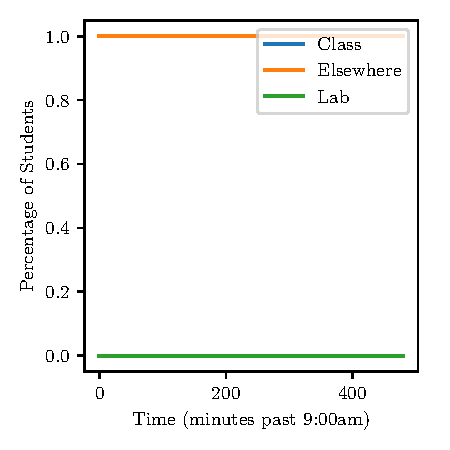
\includegraphics[width=\textwidth]{temp.pdf}
        \caption{$A_{interp.7}$}
        \label{fig:interp_degrees_7}
    \end{subfigure}
    \hfill
    \begin{subfigure}[b]{0.32\textwidth}
        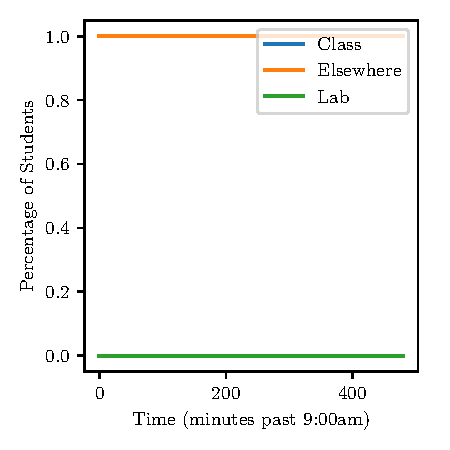
\includegraphics[width=\textwidth]{temp.pdf}
        \caption{$A_{interp.12}$}
        \label{fig:interp_degrees_12}
    \end{subfigure}
    \hfill
    \begin{subfigure}[b]{0.32\textwidth}
        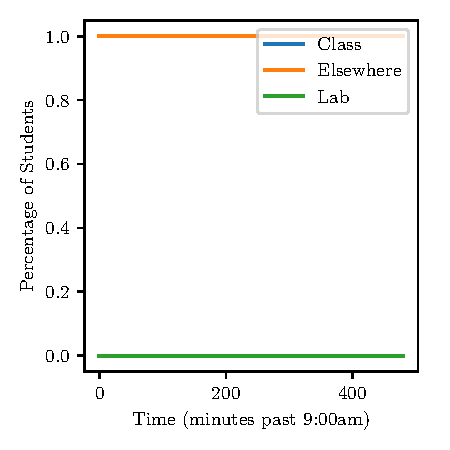
\includegraphics[width=\textwidth]{temp.pdf}
        \caption{$A_{interp.25}$}
        \label{fig:interp_degrees_25}
    \end{subfigure}
    \caption{Continuizing $A_{discontinuous}$ with various degrees of Barycentric Lagrange Interpolation 
    at the Chebyshev points. Our ensuing models use the 12-degree interpolation (bottom-left).}
    \label{fig:interp_degrees}
\end{figure}

\subsection{Incorporating Mid-Day Busy Peaks}
Since the math lab traffic peaks mid-day in what resembles
resembles a normal distribution, we simply added (or convolved) gaussian curves to $A_{EL}$ and $A_{CL}$ in $A_{interp.12}$.
Note that this modified $A$ isn't purely hour-wise periodic, but still works the same.

%% Third Section
\section{Results}
The following are the results of differing alpha matrices. All of these simulations use a sensible domain (9am–5pm). The initial values are 
given below Equation~(\ref{eq:system}), and BVP used these as initial \textit{and} final boundary conditions.

\subsection{Constant Alphas}
Simulation our model on the constant alpha matrix as given in Equation~(\ref{eq:constant_alpha}) gave the following results. See Figure ~\ref{fig:constant_alpha}.
As seen below, this timeplot doesn't have anything interesting to show.

\begin{figure}[htp]
    \centering
    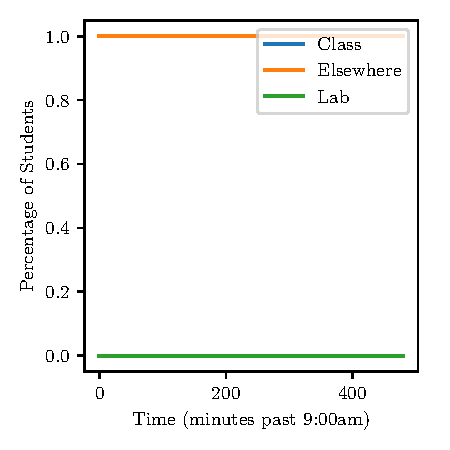
\includegraphics[width=0.45\textwidth]{temp.pdf}\hfill
    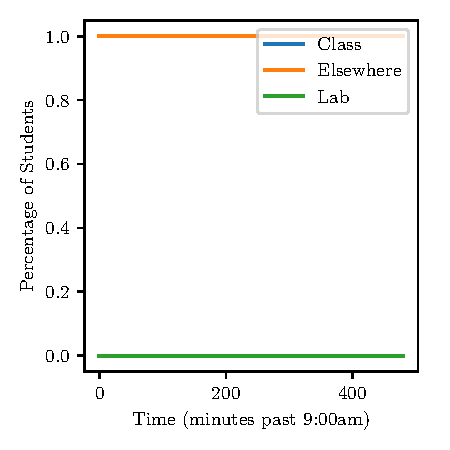
\includegraphics[width=0.45\textwidth]{temp.pdf}\hfill
    \caption{The constant alpha functions (left) along with the timeplot using IVP (right).}
    \label{fig:constant_alpha}

\end{figure}

\subsection{Discontinuous Alphas}
Simulating our model with $A_{discontinuous}$ in Equation (\ref{eq:disc}) resulted in Figure~\ref{fig:discontinuous_alpha}. 

\begin{figure}[htp]
    \centering
    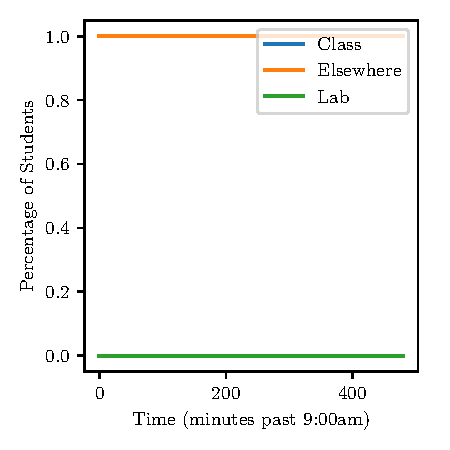
\includegraphics[width=0.45\textwidth]{temp.pdf}\hfill
    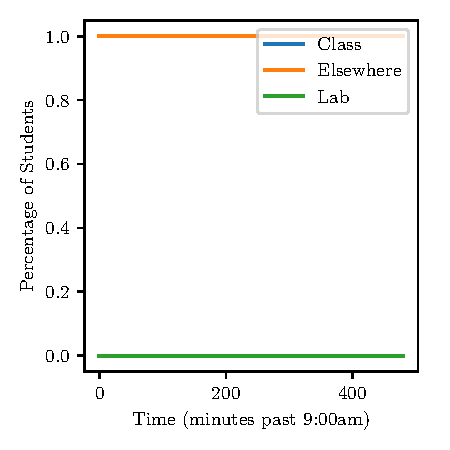
\includegraphics[width=0.45\textwidth]{temp.pdf}\hfill

    \caption{The discontinuous alpha functions (left) along with the timeplot using IVP (right).}
    \label{fig:discontinuous_alpha}

\end{figure}

The timeplot shows peaks during the transition period. We also see that the model shows majority of math students are in class throughout the day.

\subsection{Boundary Value Problem}
Simulating our model with Equation (\ref{eq:bvp}) and the given boundary conditions resulted in Figure ~\ref{fig:discontinuous_alpha_bvp}. In this one we notice the numerical software fitting
boundary conditions, which in turn makes the functions almost fit those endpoints every hour. We also see some of the plot going above $1$ and below $0$. This doesn't accurately represent the population
of math students since we can't have more than 100\% of students and less than 0\%. The peaks as seen in the normal IVP are present here, but they are more stark.
\begin{figure}[htp]
    \centering
    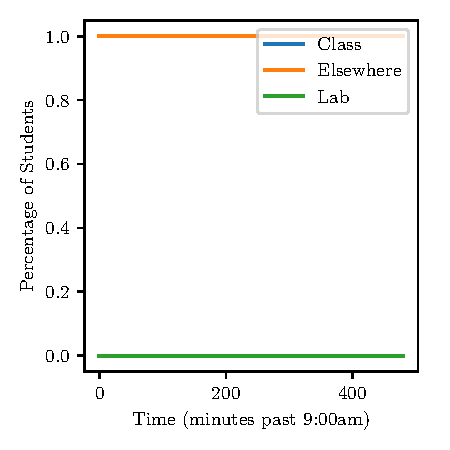
\includegraphics[width=0.5\textwidth]{temp.pdf}
    \caption{Timeplot of our ODE system with $A_{discontinuous}$, but using a BVP solver.}
    \label{fig:discontinuous_alpha_bvp}

\end{figure}

\subsection{Interpolation of Alphas}

Simulating our model using the $A_{interp.12}$ polynomial, since these ones barely dipped below zeros, yeilded the results in Figure ~\ref{fig:continuous_alpha}. The peaks once again occur, 
but the trend seems to match the polynomial in middle right of the transition matrix which is $A_{E \rightarrow C}$. This is probably the case because in reality the majority of students are 
going from elsewhere to class, but it is interesting that the lab population also takes that form because $A_{E \rightarrow C}$ isn't in the $\dot{L}$ equation.


\begin{figure}[htp]
    \centering
    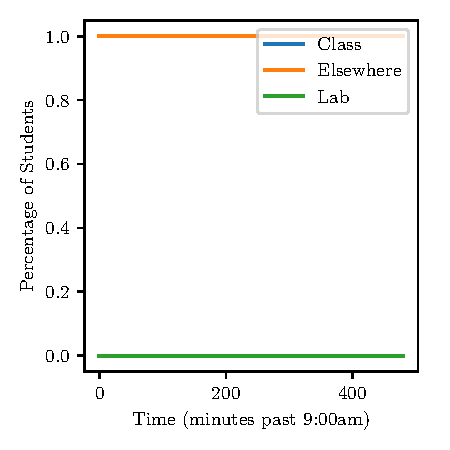
\includegraphics[width=0.3\textwidth]{temp.pdf}\hfill
    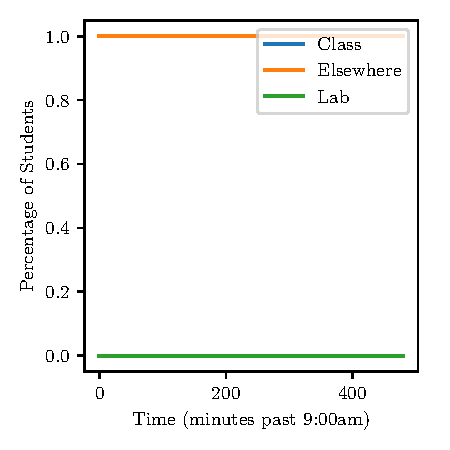
\includegraphics[width=0.3\textwidth]{temp.pdf}\hfill
    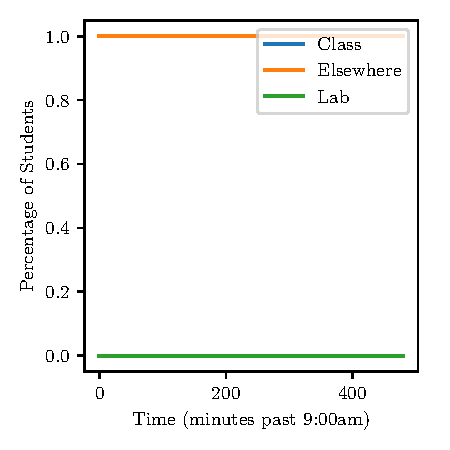
\includegraphics[width=0.3\textwidth]{temp.pdf}\hfill
    \caption{Simulating with $A_{interp.12}$ (left), giving the timeplots using both IVP (center) and BVP (right).}
    \label{fig:continuous_alpha}

\end{figure}

Finally, simulating our model on the convolved polynomial showed the results in Figure ~\ref{fig:daywise_alpha}. The IVP timeplot shows that 
the peaks will rise towards the middle of the day and then drop as the day continues. On the other hand the BVP timeplot is unaccurate because the 
scale of the percentage of students is not realisitc. It is seeming to get a lot of numerical noise and doesn't provide useful information.

\begin{figure}[htp]
    \centering
    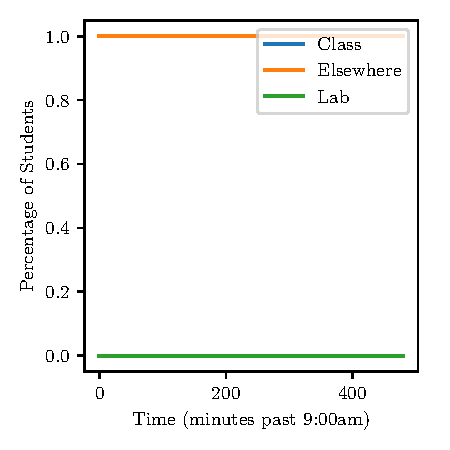
\includegraphics[width=1\textwidth]{temp.pdf}\hfill
    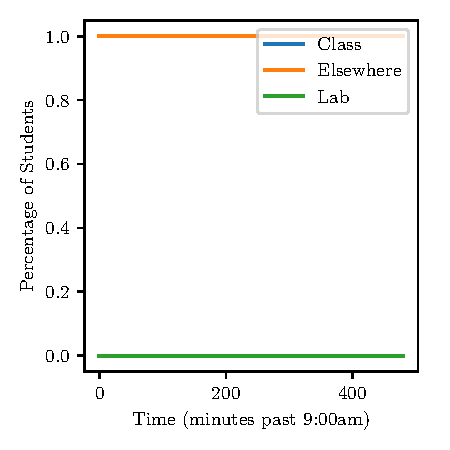
\includegraphics[width=0.45\textwidth]{temp.pdf}\hfill
    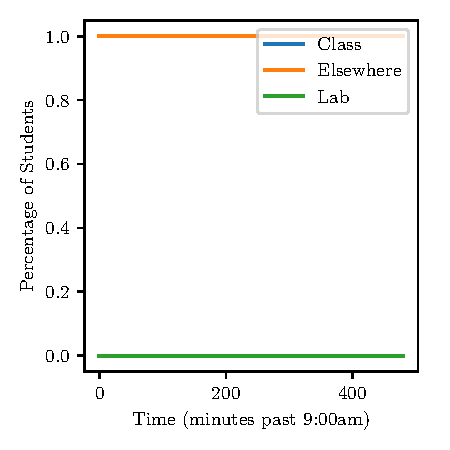
\includegraphics[width=0.45\textwidth]{temp.pdf}\hfill

    \caption{Simulating our IVP with $A_{interp.12}$ plus some gaussian terms for daily traffic (top), along with the timeplot using IVP (bottom-left) and BVP (bottom-right).
    our BVP spikes far outside our usual bounds at transitions with daily traffic.}
    \label{fig:daywise_alpha}
\end{figure}



% We then implemented the time step functions from the matrix $\A$ and got an interesting graph that changes during the class breaks. We decided to make the alpha functions
% using the time steps for around class breaks, that being from the 45 in the hour to the 5 after the hour. We are taking into account students that show up late and also students
% that show up early. Using these time functions gave us a very interesting result. As shown in the graph the population was having spikes hour to hour. Logically this makes sense 
% because the students would leave Class and then go to either the Lab or Elsewhere. The other interesting thing about this graph was that the percentage of student in class was always
% higher than the other two groups of students. 


%%Fourth Section
\section{Analysis}

\subsection{Stability}



\subsection{Pitfalls/Errors}



\section{Conclusion}



%%%%%%%%%%%%%%%%%%%%%%%%%%%%%%%%%%%%%
%% Bibliography below
%%%%%%%%%%%%%%%%%%%%%%%%%%%%%%%%%%%%%
\FloatBarrier % Keep the figures from being put after the bibliography
\newpage
%% If using bibtex, leave this uncommented
%\bibliography{refs} %if using bibtex, call your bibtex file refs.bib
\bibliographystyle{alpha}

%% If not using bibtex, comment out the previous two lines and uncomment those below
\begin{thebibliography}{99}
\bibitem{V4Textbooks} The ACME Volume 4 Textbook
\bibitem{Migration} Wang Xiang-Sheng and Wu Jianhong 2012. Seasonal migration dynamics: periodicity, transition delay and finite-dimensional reductionProc. R. Soc. A.468634–650. http://doi.org/10.1098/rspa.2011.0236
\bibitem{Population} Pierre Auger, Jean-Christophe Poggiale, Emergence of Population Growth Models: Fast Migration and Slow Growth, Journal of Theoretical Biology, Volume 182, Issue 2, 1996, Pages 99-108, ISSN 0022-5193, https://doi.org/10.1006/jtbi.1996.0145.
\end{thebibliography}

\end{document}
